\setcounter{page}{1} \pagenumbering{Alph}

% Add PDF bookmark 
\pdfbookmark[0]{Title}{Title}

\thispagestyle{empty}
\begin{flushleft} ~\\ \vspace{-12mm} \hspace{-12mm}  
\includegraphics[width=50mm]{Cover/istnewlogo} 
\vspace{10mm}
%~\\ \vspace{50mm} % gráficos
\\ \begin{center} 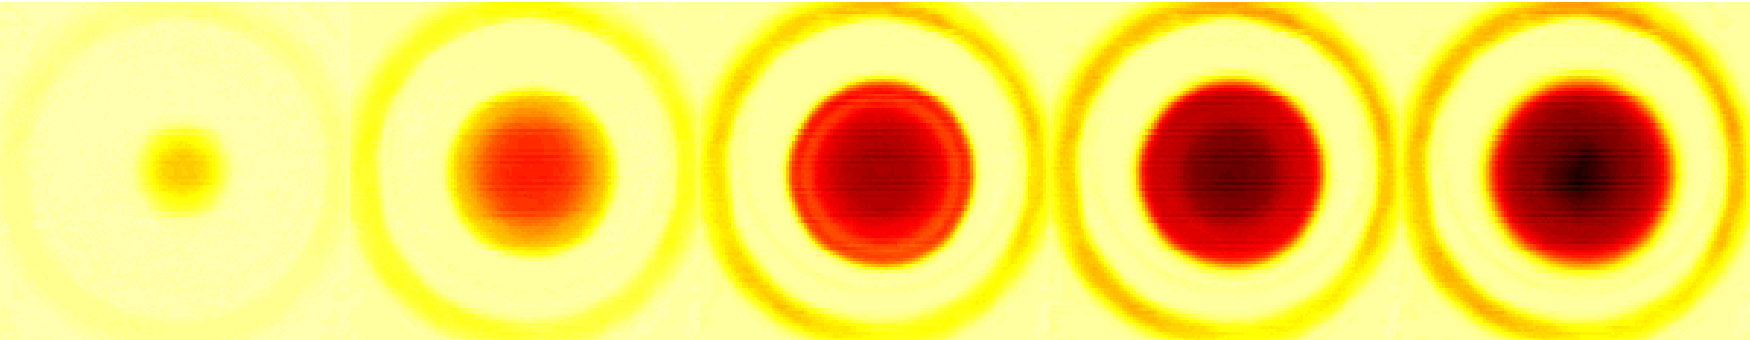
\includegraphics[width=1\linewidth]{Cover/coverimage}  \end{center} % gráficos
 \vspace{5mm}
\centering
\LARGE \textbf{Thermographical analysis of interface heat transfer mechanisms, with high temporal resolution}
%\\ \vspace{10mm}
%\Large Subtitle
\\ \vspace{15mm}
\Large \textbf{Pedro Daniel Fernandes Pontes} \\
\vspace{12mm}
\large Thesis to obtain the Master of Science Degree in
\\ \vspace{2mm}
\LARGE \textbf{Mechanical Engineering}
\\ \vspace{10mm}
\large Supervisors: Prof. Antonio Luís Nobre Moreira

Dr. Ana Sofia Oliveira Henriques Moita
\\ \vspace{15mm}
\Large \textbf{Examination Committee}
\\ \vspace{5mm}
\large Chairperson:	Prof. Viriato Sérgio de Almeida Semião \\
\large Supervisor: Dr. Ana Sofia Oliveira Henriques Moita \\
%\large Co-Supervisor: Prof. Lorem Ipsum \\
\large Member of the Committe: Prof. Edgar Caetano Fernandes \\
% Prof. Lorem Ipsum
 
\vspace{15mm}

%\Large \textbf{\todaythesis\today} \\
\Large \textbf{November 2016} \\
\let\thepage\relax
\end{flushleft}
\pagebreak


\clearpage
% Since I am using double sided pages, the second page should be white.
% Remember that when delivering the dissertation, IST requires for the cover to appear twice.

\thispagestyle{empty}
\cleardoublepage

\setcounter{page}{1} \pagenumbering{roman}

\baselineskip 18pt % line spacing: -12pt for single spacing
                   %               -18pt for 1 1/2 spacing
                   %               -24pt for double spacingnts}